% WP-C ACTOR-3; EXPLORATORY / REVIEW_BLOCKED. Not an accepted final paper section.
% Dependencies: amsmath, amssymb, booktabs, graphicx, Chinese-capable class.
% Compile from the package's paper/ directory. This fragment has NOT been compiled here.
\section{质量冲突诊断与综合评价}
\label{sec:q12-conflict}
\paragraph{证据状态}本节为探索性章节源码。上游运行尚未达到\texttt{PACKAGE\_ACCEPTED}，不得直接作为正式接受结论并入主论文。
\subsection{数据与问题分析}
使用A1、A2、A3全部272505条记录，按ID去重为261086条。A1划分为40919条拟合、10311条留出；A2与A3分别新增16104、193752条，其余为同源重叠。沿用第一问冻结归一化及CRITIC权重，原TOPSIS领域均分复算误差小于$10^{-12}$。单一总分无法区分均衡中等质量与优缺点相抵，因而保留原分并回到多维信号判断冲突。
\subsection{冲突定义}
将通用质量指标构成五维，组内继承第一问权重：
\begin{equation}
z_{ig}=\frac{\sum_{j\in G_g}w_jx_{ij}}{\sum_{j\in G_g}w_j},\qquad
v_g=\frac{\sum_{j\in G_g}w_j}{\sum_h\sum_{j\in G_h}w_j}.
\label{eq:q12-group}
\end{equation}
五维为内容价值、表达质量、整洁度、无广告程度和非重复程度。DSIR三项、无字母词及句末标点比例仍保留在原评分和对照试算中，暂不进入五维模型。这是适用性假设，不是无效指标的证明。
在A1拟合集估计$l_g=P_{20}(z_g)$、$h_g=P_{80}(z_g)$，冻结后定义
\begin{equation}
H_i=\{g:z_{ig}>h_g\},\quad L_i=\{g:z_{ig}<l_g\},\quad
I_i=\mathbf1\{H_i\ne\varnothing,L_i\ne\varnothing\}.
\label{eq:q12-conflict}
\end{equation}
据H和L是否为空形成四个互斥且穷尽的类别。分位数表示相对评价，不是语义缺陷真值或统计显著性检验。
\begin{table}[htbp]\centering
\caption{五维阈值与组权重}\label{tab:q1_conflict_thresholds}
\begin{tabular}{lrrr}
\toprule
维度 & 低阈值 & 高阈值 & 组权重 \\
\midrule
内容价值 & 0.2783 & 0.5613 & 0.2499 \\
表达质量 & 0.3578 & 0.7702 & 0.2836 \\
整洁度 & 0.2673 & 0.9884 & 0.1090 \\
无广告程度 & 0.5244 & 0.9004 & 0.1056 \\
非重复程度 & 0.6366 & 0.7838 & 0.2519 \\
\bottomrule\end{tabular}\end{table}

进一步定义强度$C_i=\max_g[(z_{ig}-h_g)/(1-h_g)]_+\max_g[(l_g-z_{ig})/l_g]_+$，广度$B_i=|H_i||L_i|/\binom52$。同一维度不能同时处于高低两端。
组内分歧另行保存：两种教育价值评分器的一高一低在A1出现415条，在全量去重中出现1402条。分类器分歧与属性权衡可能重叠，不能直接相加。
\subsection{成因分析}
区分同属性测量分歧、跨属性权衡、尺度和方向、领域或语言适用性、同源重复和领域构成变化。原文案例显示，教育产品推广可同时有内容价值与广告属性；法律机构名称的必要复述可能触发重复代理；非英语文本可能被英语流畅度拉低。15个定向案例只能说明候选机制，不能估计误判率或证明因果关系。选定16项本次无非有限值；固定模型没有随机优化器，不能虚构训练收敛不稳定。
\subsection{有限补偿综合评价候选模型}
保留原评分$Q_i^{(0)}$。对同属性分歧不武断选择某个评分器，对适用性疑点保留复核标记。对属性权衡构造偏好权重不确定集合
\begin{equation}
\mathcal W_\lambda=\{(1-\lambda)v+\lambda p:p\ge0,\ \sum_gp_g=1\},\quad
Q_i^{\mathrm{cand}}=100\min_{a\in\mathcal W_\lambda}\sum_ga_gz_{ig}.
\label{eq:q12-robust}
\end{equation}
令$M_i=\sum_gv_gz_{ig}$、$m_i=\min_gz_{ig}$。线性目标在单纯形顶点上取得最小值，故
\begin{equation}
Q_i^{\mathrm{cand}}(\lambda)=100[(1-\lambda)M_i+\lambda m_i],\qquad
Q_i^{\mathrm{cand}}-100M_i=-100\lambda(M_i-m_i).
\label{eq:q12-closed}
\end{equation}
当$0\le\lambda\le1$时，该函数处于$[100m_i,100M_i]$内，对每个维度单调不减。相同维度值$c$对应$100c$。该规则连续应用于所有文本，不因离散冲突标签跨阈产生突然扣分。取$\lambda=0.25$仅为展示，并比较0、0.1、0.25、0.5；没有标签时不能称其最优。该建议交由WP-B审议，不能自动替换原评分。
\subsection{结果与扩展检验}
\begin{table}[htbp]\centering
\caption{候选冲突的分层统计}\label{tab:q1_conflict_coverage}
\begin{tabular}{lrrr}
\toprule
分区 & 样本数 & 候选冲突数 & 候选冲突率\% \\
\midrule
A1\_full & 51230 & 15124 & 29.5218 \\
A1\_holdout & 10311 & 3039 & 29.4734 \\
A2\_overlap & 1419 & 798 & 56.2368 \\
A2\_new & 16104 & 9408 & 58.4203 \\
A3\_overlap & 10000 & 3347 & 33.4700 \\
A3\_new & 193752 & 65795 & 33.9584 \\
union\_unique & 261086 & 90327 & 34.5966 \\
\bottomrule\end{tabular}\end{table}

A1四类依次为15124、14958、14439、6709条。arxiv在A1中的候选冲突率56.24\%，新增58.42\%；github分别33.47\%、33.96\%。新增集不是独立真值，另外五域没有扩展验证。全量冲突率34.60\%按A1领域比例重加权后为29.67\%，总体增幅主要来自领域构成变化。
\begin{figure}[htbp]\centering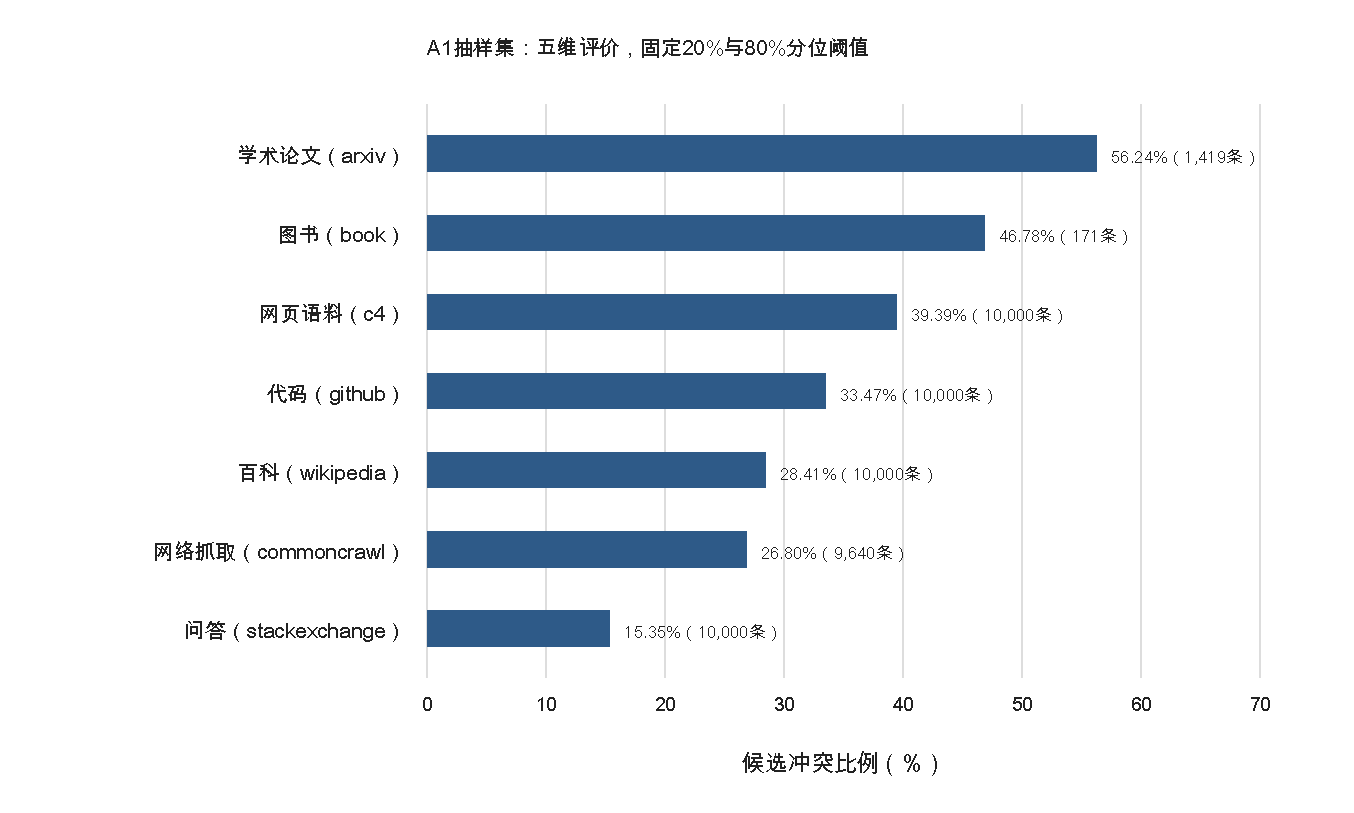
\includegraphics[width=.95\linewidth]{figures/fig1_domain_conflict.pdf}\caption{A1七域候选冲突率及样本量，阈值由A1拟合集冻结。}\label{fig:q12-domains}\end{figure}
\begin{table}[htbp]\centering
\caption{有限补偿候选评分}\label{tab:q1_resolution_scores}
\begin{tabular}{lrrrr}
\toprule
分区 & 原TOPSIS均分 & 五维加权均分 & 候选稳健均分 & 相对五维基线变化 \\
\midrule
A1\_full & 60.9471 & 58.6944 & 52.8212 & -5.8733 \\
A1\_holdout & 61.0370 & 58.7548 & 52.8643 & -5.8905 \\
A2\_new & 63.4735 & 76.5370 & 72.2455 & -4.2915 \\
A3\_new & 51.6887 & 46.9338 & 40.4316 & -6.5022 \\
union\_unique & 54.2323 & 51.0674 & 44.8250 & -6.2424 \\
\bottomrule\end{tabular}\end{table}

与原TOPSIS的分差混合了指标集合和聚合方式变化；只能将相对五维加权均分的变化归于有限补偿参数。得分降低不意味着准确率提高。arxiv新增候选分与原分的Spearman相关为0.6105，说明排序改变不能忽略。
\subsection{敏感性与限制}
从P10/P90改为P25/P75，A1冲突率从9.09\%变为41.23\%，arxiv新增从3.89\%变为79.07\%；领域相对排序也改变，不能声称单阈值结论稳健。广告指标的相对低分位与原始分类器偏向广告不同：高内容价值/相对低无广告在A1有1884条，换为广告logit大于无广告logit仅310条。
\begin{figure}[htbp]\centering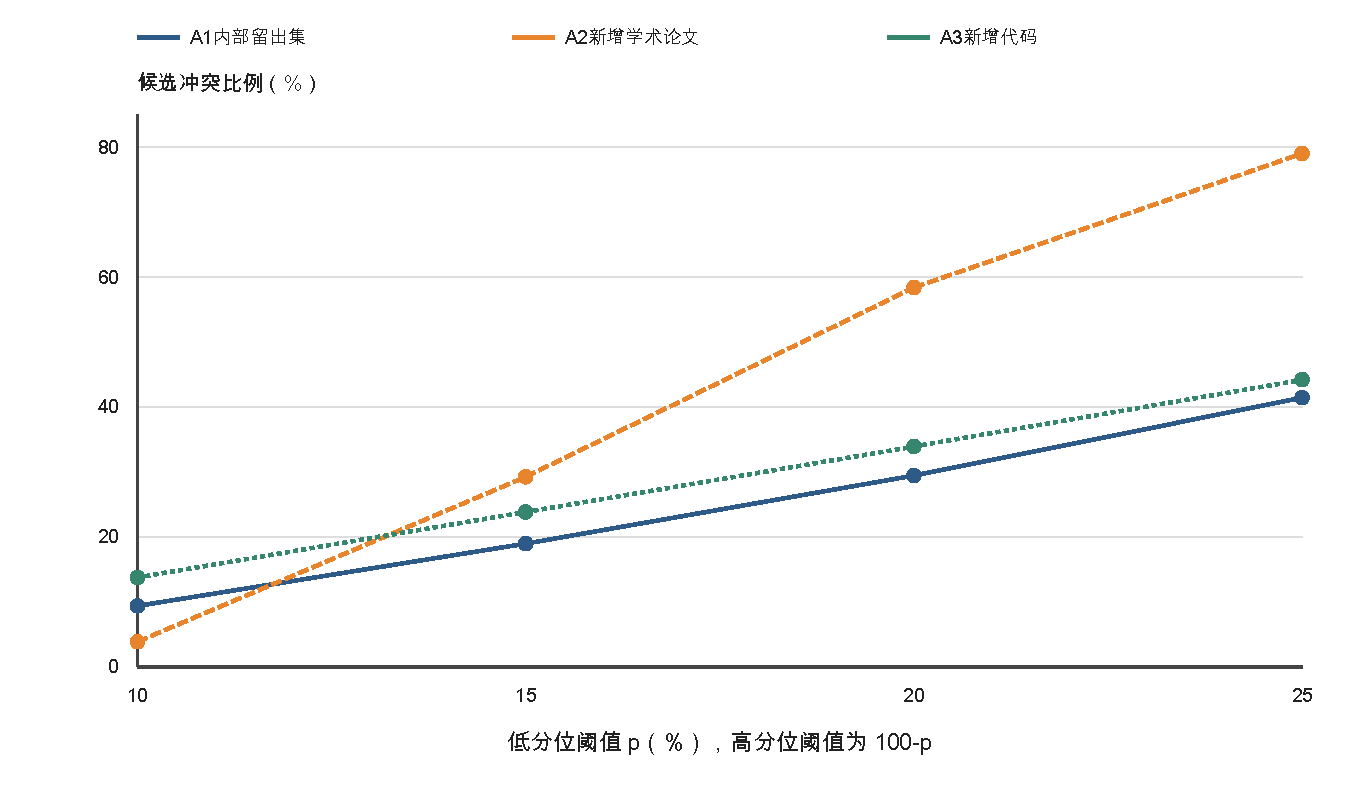
\includegraphics[width=.95\linewidth]{figures/fig2_threshold_sensitivity.pdf}\caption{冻结A1拟合参照的阈值敏感性。}\label{fig:q12-threshold}\end{figure}
\begin{figure}[htbp]\centering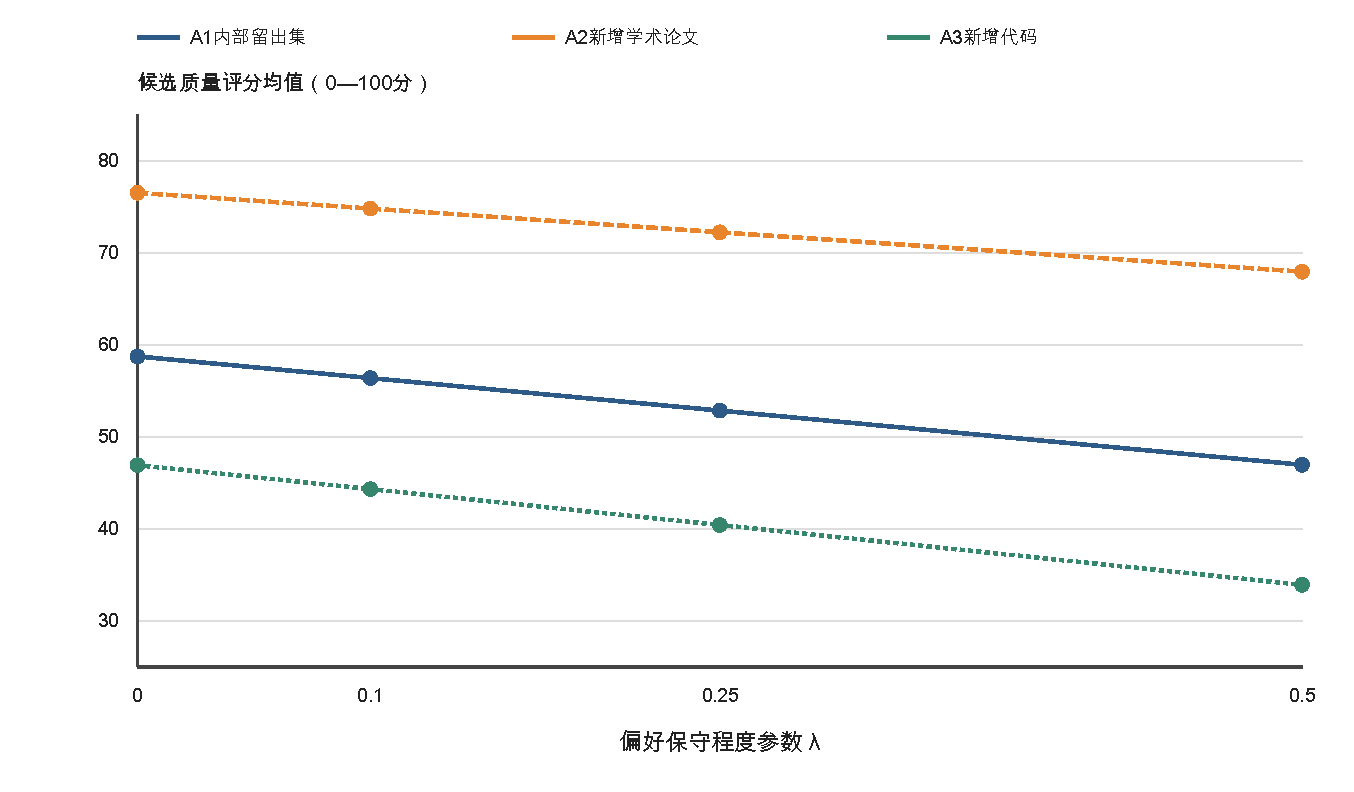
\includegraphics[width=.95\linewidth]{figures/fig3_compensation_sensitivity.pdf}\caption{偏好保守程度对候选均分的影响，不代表预测准确率。}\label{fig:q12-lambda}\end{figure}
已核对复算、重复、类别穷尽性、候选模型单调性和闭式解。正式bootstrap、权重扰动和文本对排名反转须在G2通过后执行；当前只完成相应脚本及合成接口测试，不报告虚构区间。无人工真值或下游Loss证据，83条分层复核清单保持未标注。正式发布需ACTOR-1复核、ACTOR-2集成及跨包发布流程。
